% PrototypeComparison.tex
\section{Comparative Analysis}

To assess the accuracy of the developed simulation model, results from a full simulation run were compared against experimental data collected using the same sensor topology and an equivalent arc motion sequence.

Figure~\ref{fig:ModelandPhysicalResultsComparison} presents a side-by-side comparison:
\begin{itemize}
    \item \textbf{Left:} Simulated illumination per sensor, expressed as the percentage of total emitted rays that intersected with each sensor area, plotted against the arc rotation angle.
    \item \textbf{Right:} Experimentally measured voltages from each physical sensor during the emitter's arc sweep. Signals have been filtered to reduce noise and highlight the response envelope.
\end{itemize}
\subsection*{Key Observations}
\begin{enumerate}
    \item \textbf{Overall Response Pattern:} Both plots show a clear progression of peak response across the sensor array. Sensor A2 activates first, followed by A1, A0, and then A3, which is consistent with the expected sequence during the rotation.
    
    \item \textbf{Peak Alignment:} The positions of the peak responses in the simulated and experimental plots align closely, suggesting that the source plane's movement and orientation in the simulation accurately reflects the RED testbench's real process.

\end{enumerate}
 \begin{landscape}
    \begin{figure}[htbp] %h-ere t-op b-ottom p-page (separte) -good to allow all htbp to give the compiler more options
        \centering
        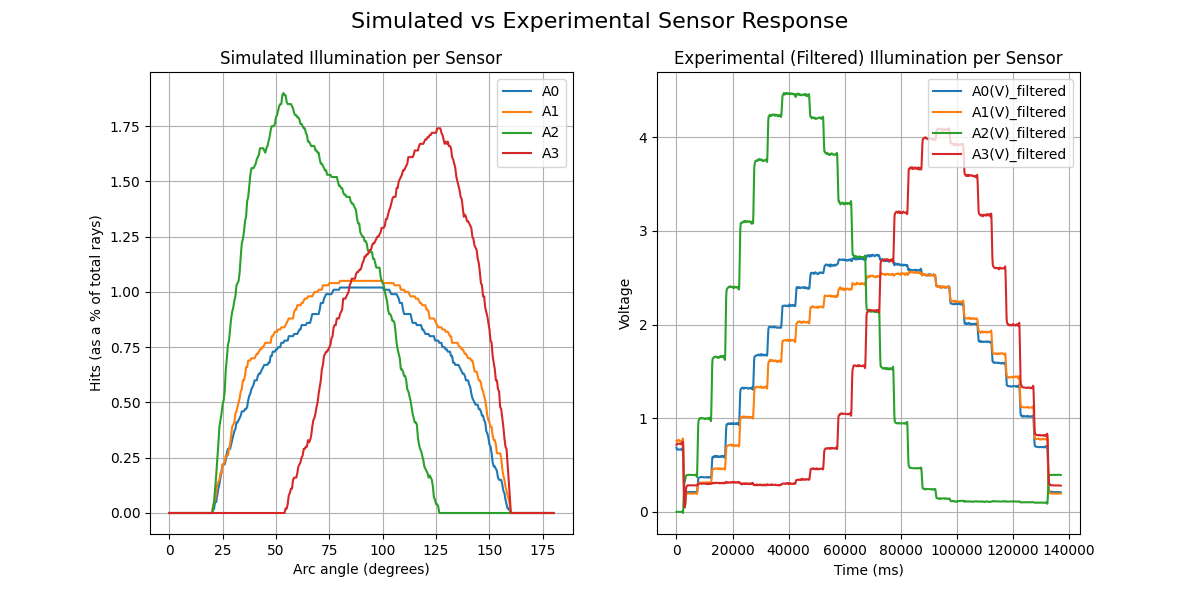
\includegraphics[width=1.4\textwidth]{chapters/results/images/Comparison_plot.png} % change {path}
        \caption{Model and Physical Results Comparison}       % change {caption}
        \label{fig:ModelandPhysicalResultsComparison}            % change label - used for reference in text
    \end{figure}
 \end{landscape}

The simulation and hardware behave in the same way, sensors are gradually illuminated and fade out as expected. The simulation appears to be handling the geometry correctly, and the physical sensor design works as intended.


\subsection*{Interpretation}
This result provides strong validation for:
\begin{itemize}
    \item The geometric modelling of planes, areas, and ray emission in the simulation framework.
    \item The arc rotation logic, particularly the ``rigid arc'' strategy where the plane consistently faces the origin.
    \item The accuracy of the designed sensor layout and aperture configuration.
\end{itemize}


% Example figure jpg
%
% \begin{figure}[htb]
%     \centering
%     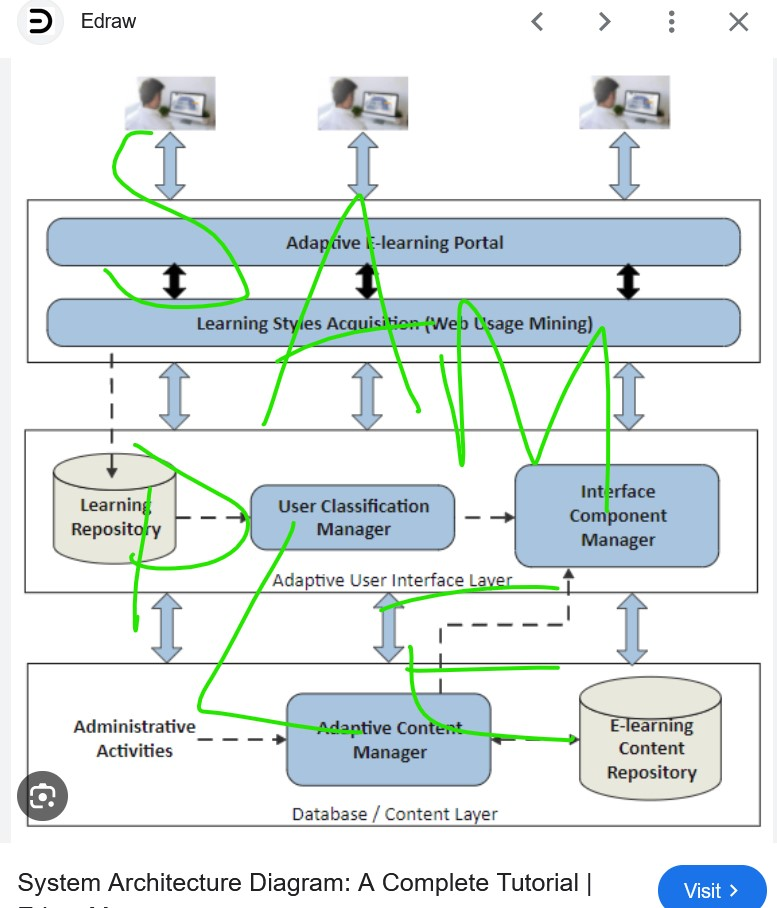
\includegraphics[width=1\textwidth]{figures/results/system_architecture.jpg}
%     \caption{Overall System Performance Analysis}
%     \label{fig:systemPerformance}
% \end{figure}

% Example listing (such as text output from console)
% \begin{figure}[H]
%     \begin{lstlisting}[style=cstyle]
%     // Environmental test results
%     // Temperature, ambient light, and vibration effects
%     \end{lstlisting}
%     \caption{Environmental Testing Results}
%     \label{lst:EnvironmentalTests1}
%     \end{figure}